\documentclass[11pt]{article}
\usepackage{acl}
\usepackage{times}
\usepackage{latexsym}
\usepackage[T1]{fontenc}
\usepackage[utf8]{inputenc}
\usepackage{microtype}
\usepackage{graphicx}
\usepackage{booktabs}
\usepackage{xcolor}
\usepackage{hyperref}

% Reduce excessive hyphenation in narrow ACL columns
\tolerance=1500
\emergencystretch=1.5em
\hyphenpenalty=600

\graphicspath{{../figures/}{../outputs/figures/}}

\title{Mining Actionable Suggestions from High-Rated Hotel Reviews:\\A Cross-Domain Transfer Learning Approach}

\author{
  Chase Sun \and Clara Yang \and Leah Luo \and Xiayi Zhu \\
  UCL School of Management \\
  MSIN0221 Natural Language Processing}

\begin{document}
\maketitle

% ── Contribution table (required by brief) ──
\begin{table*}[t]
\centering\small
\begin{tabular}{lp{12cm}}
\toprule
\textbf{Member} & \textbf{Contribution} \\
\midrule
Chase & Pipeline architecture, preprocessing, BERT fine-tuning, reproducibility \\
Clara & EDA, report drafting (Methods, Results, Data) \\
Leah  & Annotation guidelines, BERTopic clustering, report (Intro, Related Work, Discussion) \\
Xiayi & Baselines (regex, TF-IDF+LR), error analysis, manual validation, presentation \\
\bottomrule
\end{tabular}
\end{table*}

\begin{abstract}
To what extent can NLP models detect actionable improvement
suggestions within high-star hotel reviews? We address this
question by applying suggestion mining---a sentence-level binary
classification task---to 70,085 sentences extracted from 8,571
four- and five-star TripAdvisor reviews of Marina Bay Sands,
Singapore. We compare three model tiers of increasing complexity:
a regex baseline, a TF-IDF with logistic regression classifier,
and a BERT model with two-stage fine-tuning. All models are first
trained or evaluated on the SemEval-2019 Task~9 dataset from
software forums, then tested on 80 human-annotated hotel review
sentences to measure cross-domain transfer. We further apply
BERTopic clustering to characterise the thematic content of
predicted suggestions. BERT with two-stage fine-tuning achieves
the best suggestion-class F1 of 0.581 on the hotel domain,
approximately doubling the cross-domain-only result (0.286).
Domain adaptation proves essential: without in-domain fine-tuning,
learned models drop by up to 0.43 suggestion-class F1. Thematic
analysis shows that room amenities
and facilities account for over a third of detected suggestions.
\end{abstract}

\section{Introduction}

Hotel reviews on platforms such as TripAdvisor are widely used by travellers and
hotel operators alike. Reviews with four or five stars are generally assumed to
express satisfaction, yet they frequently contain concrete suggestions for
improvement embedded within otherwise positive text. A guest who rates a hotel
five stars may still write, ``I wish the breakfast had more vegetarian
options.'' Standard sentiment analysis classifies such reviews as positive,
missing the constructive content within them.

Suggestion mining is the task of identifying sentences that propose an
improvement, give advice, or recommend an action \citep{negi2018open}. Framed as
sentence-level binary classification, it distinguishes suggestions from
non-suggestions. The task was formalised in the SemEval-2019 Task~9 shared task
\citep{negi2019semeval}, which provided labelled data from software developer
forums. That shared task demonstrated that BERT-based models achieved the best
performance for in-domain suggestion detection but also revealed that
cross-domain transfer---applying a model trained on one domain to
another---remains a challenge \citep{park2019bert}.

While SemEval-2019 Task~9 Subtask~B evaluated cross-domain
transfer to hotel reviews, no prior work combines
domain-adapted annotation guidelines, a multi-tier model
comparison, and thematic analysis for suggestion mining in
high-rated hotel reviews. Hotel reviews differ from software forums in
vocabulary, sentence structure, and the way suggestions are expressed:
software forum users write explicit feature requests (``The API should support
batch uploads''), while hotel guests embed suggestions within narrative
descriptions (``The room was lovely but the pillows could be firmer''). This
domain shift makes direct transfer from existing datasets non-trivial, and
raises the question of how much domain-specific adaptation is needed.

Our research question is: \textbf{To what extent can NLP models detect
actionable improvement suggestions within high-star hotel reviews?}

We address this question through four contributions:
\begin{itemize}
  \item \textbf{Domain-adapted annotation guidelines} for identifying
  suggestions in hotel reviews, with inter-annotator agreement measured on a
  calibration sample of 100 sentences.
  \item \textbf{A three-tier model comparison}---regex baseline, TF-IDF with
  logistic regression (TF-IDF~+~LR) baseline, and BERT classifier---that
  quantifies the value of increasingly rich representations for suggestion
  detection.
  \item \textbf{Two-stage fine-tuning} of BERT: first on the SemEval-2019
  training data, then on annotated hotel review sentences, with a cross-domain
  evaluation that measures the performance delta between in-domain and
  cross-domain settings.
  \item \textbf{BERTopic-based thematic analysis} of extracted suggestions,
  grouping them into hotel-relevant categories (room, food and beverage, service,
  facilities, location, value).
\end{itemize}

\section{Related Work}

\paragraph{Suggestion mining.}
\citet{negi2018open} formalised suggestion mining as the task of identifying
sentences that express a suggestion, defined as a sentence that proposes an
improvement, gives advice, or recommends a course of action. Earlier approaches
relied on hand-crafted rules targeting modal verbs and imperative constructions
\citep{negi2017distant}. The SemEval-2019 Task~9 shared task
\citep{negi2019semeval} established benchmark datasets and attracted 33
participating teams. The best-performing systems used BERT-based architectures,
with the top system achieving 78.1\% suggestion-class F1 on Subtask~A
(in-domain). Subtask~B required cross-domain generalisation from software forums
to hotel reviews, where performance dropped for many systems, indicating that
domain shift is a core challenge in suggestion mining.

\paragraph{Domain adaptation and BERT fine-tuning.}
Pre-trained language models such as BERT \citep{devlin2019bert} learn general
linguistic representations that can be adapted to downstream tasks via
fine-tuning. However, fine-tuned models can be brittle when the target domain
differs from the training domain. \citet{park2019bert} showed that BERT is
unstable for out-of-domain suggestion mining, with high variance across runs on
cross-domain data. \citet{prasanna2019zoho} addressed this by applying
tri-training, a semi-supervised bootstrapping approach, to label target-domain
data without manual annotation, achieving 81.94\% suggestion-class F1 on the
cross-domain subtask. These findings motivate our two-stage fine-tuning
strategy: first training on the larger SemEval dataset for task knowledge, then
adapting to hotel-domain data.

\paragraph{Sentiment analysis versus suggestion mining.}
Suggestion mining is distinct from sentiment analysis. A five-star review is
positive in sentiment but may contain sentences that propose improvements.
Aspect-based sentiment analysis identifies opinions about specific features
(e.g.\ ``the pool was clean''), but does not distinguish between descriptive
praise and constructive suggestions (e.g.\ ``they should heat the pool''). Our
work targets this gap by extracting the subset of sentences that contain
improvement-oriented content, regardless of overall sentiment, and grouping
them thematically using BERTopic \citep{grootendorst2022bertopic} to produce
actionable insights for hotel management.

\section{Data}

\subsection{Marina Bay Sands Review Dataset}

We collected 10,232 English-language reviews of Marina Bay
Sands, Singapore from TripAdvisor, spanning January 2014 to
October 2022. We filtered for four- and five-star reviews, targeting
reviews likely to contain improvement suggestions embedded within
positive text. After removing null entries, 8,571
reviews remained: 2,414 four-star and 6,157 five-star.

We segmented reviews into sentences using the spaCy
\texttt{en\_core\_web\_sm} model \citep{honnibal2020spacy} and
applied three sequential cleaning steps to the 72,391 segmented
sentences: (1)~a language filter removing 1 non-English sentence,
(2)~exact deduplication removing 1,137 duplicates, and (3)~a
length filter removing 1,168 sentences outside the 4--100 token
range. After all preprocessing, 70,085
sentences remained, with a median length of 15 tokens and a mean
of 8.4 sentences per review. Table~\ref{tab:mbs-stats}
summarises the dataset statistics.

\begin{table}[t]
\centering\small
\caption{MBS dataset statistics.}
\label{tab:mbs-stats}
\begin{tabular}{lr}
\toprule
\textbf{Statistic} & \textbf{Value} \\
\midrule
Raw reviews            & 10,232 \\
After 4--5 star filter & 8,571  \\
Four-star reviews      & 2,414  \\
Five-star reviews      & 6,157  \\
Sentences after preprocessing & 70,085 \\
Median sentence length (tokens) & 15 \\
Mean sentences per review & 8.4 \\
\bottomrule
\end{tabular}
\end{table}

\subsection{SemEval-2019 Task 9 Dataset}

We use the publicly available SemEval-2019 Task~9 Subtask~A dataset
\citep{negi2019semeval}, collected from the Uservoice software feedback forum.
The SemEval training set contains 8,500 sentences (2,085
suggestions, 6,415 non-suggestions; 24.5\% suggestion rate). The
SemEval test set contains 833 sentences (87 suggestions, 746
non-suggestions; 10.4\% suggestion rate). This class imbalance,
particularly in the SemEval test set, motivates our use of
suggestion-class
F1 rather than accuracy as the primary evaluation metric.

The SemEval dataset differs from our MBS sentences in several respects. Software
forum posts tend to be explicit feature requests using modal verbs (``The system
should allow\ldots''), while hotel review suggestions are often implicit,
embedded within descriptive or comparative language (``I wish the breakfast
had\ldots''). Sentence lengths and vocabulary also differ: the SemEval data
contains technical terms absent from hospitality reviews. These differences
constitute the domain shift that our cross-domain evaluation measures.

\begin{table}[t]
\centering\small
\caption{SemEval-2019 Task~9 dataset statistics.}
\label{tab:semeval-stats}
\begin{tabular}{lrrrr}
\toprule
\textbf{Split} & \textbf{Total} & \textbf{Sugg.} & \textbf{Non-sugg.} & \textbf{Rate} \\
\midrule
Training & 8,500 & 2,085 & 6,415 & 24.5\% \\
Test     &   833 &    87 &   746 & 10.4\% \\
\bottomrule
\end{tabular}
\end{table}

\subsection{Annotation}

We developed annotation guidelines adapted from the SemEval-2019
task definition \citep{negi2019semeval,negi2018open}, with
extensions for hotel-domain edge cases such as comparative
suggestions, implicit improvement requests, and the distinction
between complaints and concrete suggestions.

\paragraph{Calibration round.} All four annotators independently
  labelled the same MBS calibration sample of 100 sentences. To
  increase the proportion of informative examples, we used signal
  enrichment: 50\% of the sample was drawn from sentences
  containing suggestion-signal keywords (modal verbs, imperatives,
  conditionals), and 50\% was drawn randomly. Inter-annotator
  agreement was fair: Fleiss' $\kappa$ = 0.379. Pairwise Cohen's
  $\kappa$ ranged from 0.212 to 0.672 (mean 0.426). The highest
  pairwise agreement (0.672) occurred between two annotators who
  most consistently distinguished complaints from suggestions; the
  lowest (0.212) reflected differing thresholds for implicit
  suggestions. The moderate overall agreement is consistent with
  the subjective nature of suggestion boundaries reported by
  \citet{negi2018open}.

\paragraph{Disagreement resolution.} Sentences with majority
  agreement (3 or 4 of 4 annotators) received the majority label.
  Of the 100 calibration sentences, 11 produced 2-vs-2 ties; these
  were resolved by group discussion. Most ties involved sentences
  where negative sentiment co-occurred with modal verbs (e.g.\
  ``I would definitely stay again''), which annotators initially
  split on. After calibration, guidelines were revised to clarify
  two recurring edge cases: complaints without actionable direction
  and informational statements versus guest-directed advice.

\paragraph{Split annotation.} After calibration, 300 additional
  sentences were divided into four batches of 75, with each
  annotator labelling one batch independently. Combined with the
  100 calibration sentences, the MBS annotated set contains 400
  sentences: 73 suggestions (18.25\%) and 327 non-suggestions
  (81.75\%). The suggestion rate is lower than the SemEval training
  set (24.5\%), reflecting the less directive language typical of
  hotel reviews.

\paragraph{Train/test split.} The MBS annotated set was split
  80/20 (stratified by label) into an MBS train split of 320
  sentences (58 suggestions, 18.1\%) and an MBS test split of 80
  sentences (15 suggestions, 18.8\%).

\section{Methods}

\subsection{Task Formulation}

We framed suggestion mining as binary sentence classification:
each sentence was labelled as suggestion~(1) or
non-suggestion~(0). Classification operated at the sentence
level, consistent with the SemEval-2019 task definition. We did
not use review-level context; each sentence was classified
independently.

\subsection{Tier 1: Regex Baseline}

The regex baseline classified a sentence as a suggestion if it
matched any of 24 hand-crafted regular expression patterns.
These patterns covered three categories:
modal suggestions (e.g.\ \texttt{\textbackslash bshould\textbackslash b},
\texttt{\textbackslash bcould improve\textbackslash b}, \texttt{\textbackslash
bneed to\textbackslash b}), imperatives (e.g.\ \texttt{\textbackslash
bplease\textbackslash b}, \texttt{\textbackslash brecommend\textbackslash b},
\texttt{\textbackslash bconsider\textbackslash b}), and conditionals (e.g.\
\texttt{\textbackslash bi wish\textbackslash b}, \texttt{\textbackslash bit
would be nice\textbackslash b}, \texttt{\textbackslash bhopefully\textbackslash
b}). Matching was case-insensitive. This baseline established a
performance floor and demonstrated the limitations of surface
patterns---for instance, ``We would recommend this hotel to
anyone'' matches the modal pattern but is not a suggestion.

\subsection{Tier 2: TF-IDF + LR Baseline}

The TF-IDF~+~LR baseline used a TF-IDF vectoriser (unigrams
and bigrams, maximum 10,000 features, minimum document
frequency~2, sublinear term-frequency scaling) followed by
logistic regression (regularisation $C=1.0$, balanced class
weights, maximum 1,000 iterations), implemented in scikit-learn
\citep{pedregosa2011scikit}. The model was trained on the SemEval training set. Balanced
class weights addressed the class imbalance by upweighting the
minority suggestion class. This baseline showed the value of
learned features over hand-crafted rules while remaining
interpretable and fast to train.

\subsection{Tier 3: BERT Classifier with Two-Stage Fine-Tuning}

Our primary model was \texttt{bert-base-uncased}
\citep{devlin2019bert}, a 110-million-parameter pre-trained
transformer implemented via the HuggingFace Transformers library
\citep{wolf2020transformers}, fine-tuned for binary
classification with an additional linear output layer.

\paragraph{Stage~1: SemEval fine-tuning.} We fine-tuned on the SemEval training
  set (8,500 sentences), using a 90/10 stratified train/validation split.
  Sentences were tokenised with a maximum length of 128 tokens. Training used the
  AdamW optimiser \citep{loshchilov2019adamw} with learning rate
  $2 \times 10^{-5}$, batch size~16,
  3~epochs, linear warmup over 10\% of training steps, and weight decay~0.01. We
  selected the checkpoint with the best macro~F1 on the validation split. On the
  SemEval validation split, BERT stage-1 achieved macro~F1 of 0.886 and
  suggestion-class~F1 of 0.828.

\paragraph{Stage~2: MBS domain adaptation.} Starting from the stage-1
  checkpoint, we further fine-tuned on the MBS train split, using an 85/15
  stratified train/validation split. The learning rate was reduced to $1 \times
  10^{-5}$ to avoid overwriting task knowledge learned in stage~1. All other
  hyperparameters remained the same. This two-stage approach followed the principle
  of progressive fine-tuning: pre-trained representations $\rightarrow$
  task-specific fine-tuning $\rightarrow$ domain-specific adaptation.

All training was performed on Apple Silicon (MPS backend) with a fixed random
seed of 42. Hyperparameters follow \citet{devlin2019bert}.

\subsection{Insight Generation: BERTopic Clustering}

To transform binary predictions into thematic insights, we
applied BERTopic \citep{grootendorst2022bertopic} to all
sentences predicted as suggestions by BERT stage-2. Sentence
embeddings were computed with \texttt{all-MiniLM-L6-v2}
\citep{reimers2019sentence}. Dimensionality reduction used UMAP
\citep{mcinnes2018umap} (5~components, 15~neighbours, cosine
metric, minimum distance~0.0). Clustering used HDBSCAN
\citep{campello2013hdbscan} (minimum cluster size~5). Topic
representations were extracted via a class-based TF-IDF
procedure. The number of topics was determined automatically.

As a complementary analysis, we applied keyword-based aspect
grouping to the same set of predicted suggestions. Six
hotel-relevant aspects were defined: room, food and beverage,
service, facilities, location, and value. Each sentence was
assigned to the aspect whose keywords appeared most frequently,
or to ``other'' if no keywords matched. This provided a coarser
but more interpretable categorisation than BERTopic.

\subsection{Evaluation}

Our primary metric is suggestion-class~F1, computed on label~1 only. We also
report precision, recall, and macro~F1. All models are evaluated on both the
SemEval test set (in-domain evaluation) and the MBS test split (cross-domain
evaluation). The difference between in-domain and cross-domain
suggestion-class~F1---the performance delta---quantifies the domain gap.
We do not perform a separate manual validation step on the full
MBS predictions. This limitation is discussed in
Section~6.3.

\section{Results}

\subsection{Model Comparison}

Table~\ref{tab:results} reports suggestion-class F1 for each
model on both datasets. On the SemEval test set, BERT stage-1
achieves the highest suggestion-class F1 (0.716), followed by
TF-IDF~+~LR (0.596) and the regex baseline (0.386). Each tier
improves over the previous, confirming that learned
representations outperform hand-crafted patterns for in-domain
suggestion detection.

\begin{table}[t]
\centering\footnotesize
\caption{Suggestion-class metrics. P = precision, R = recall.
  $\Delta$ = MBS F1 $-$ SemEval F1.}
\label{tab:results}
\begin{tabular}{l@{\hskip 4pt}ccc@{\hskip 6pt}cccc}
\toprule
& \multicolumn{3}{c}{\textbf{SemEval}}
& \multicolumn{3}{c}{\textbf{MBS}} & \\
\cmidrule(lr){2-4} \cmidrule(lr){5-7}
\textbf{Model} & P & R & F1 & P & R & F1
  & $\Delta$ \\
\midrule
Regex      & .405 & .368 & .386 & .421 & .533 & .471
  & $+$.09 \\
TF-IDF+LR  & .486 & .770 & .596 & .333 & .133 & .190
  & $-$.41 \\
BERT s-1   & .624 & .839 & .716 & .500 & .200 & .286
  & $-$.43 \\
BERT s-2   & .513 & .908 & .656 & .563 & .600 & .581
  & $-$.08 \\
\bottomrule
\end{tabular}
\end{table}

On the MBS test split, BERT stage-2 achieves the best
suggestion-class F1 (0.581), approximately doubling the stage-1
result (0.286). The two-stage fine-tuning improves both precision (0.500
$\rightarrow$ 0.563) and recall (0.200 $\rightarrow$ 0.600) on
MBS, indicating that domain-specific training helps the model
recognise hotel-style suggestion language.
Figure~\ref{fig:cm-s2} shows the confusion matrix for BERT
stage-2 on the MBS test split.

\begin{figure}[t]
\centering
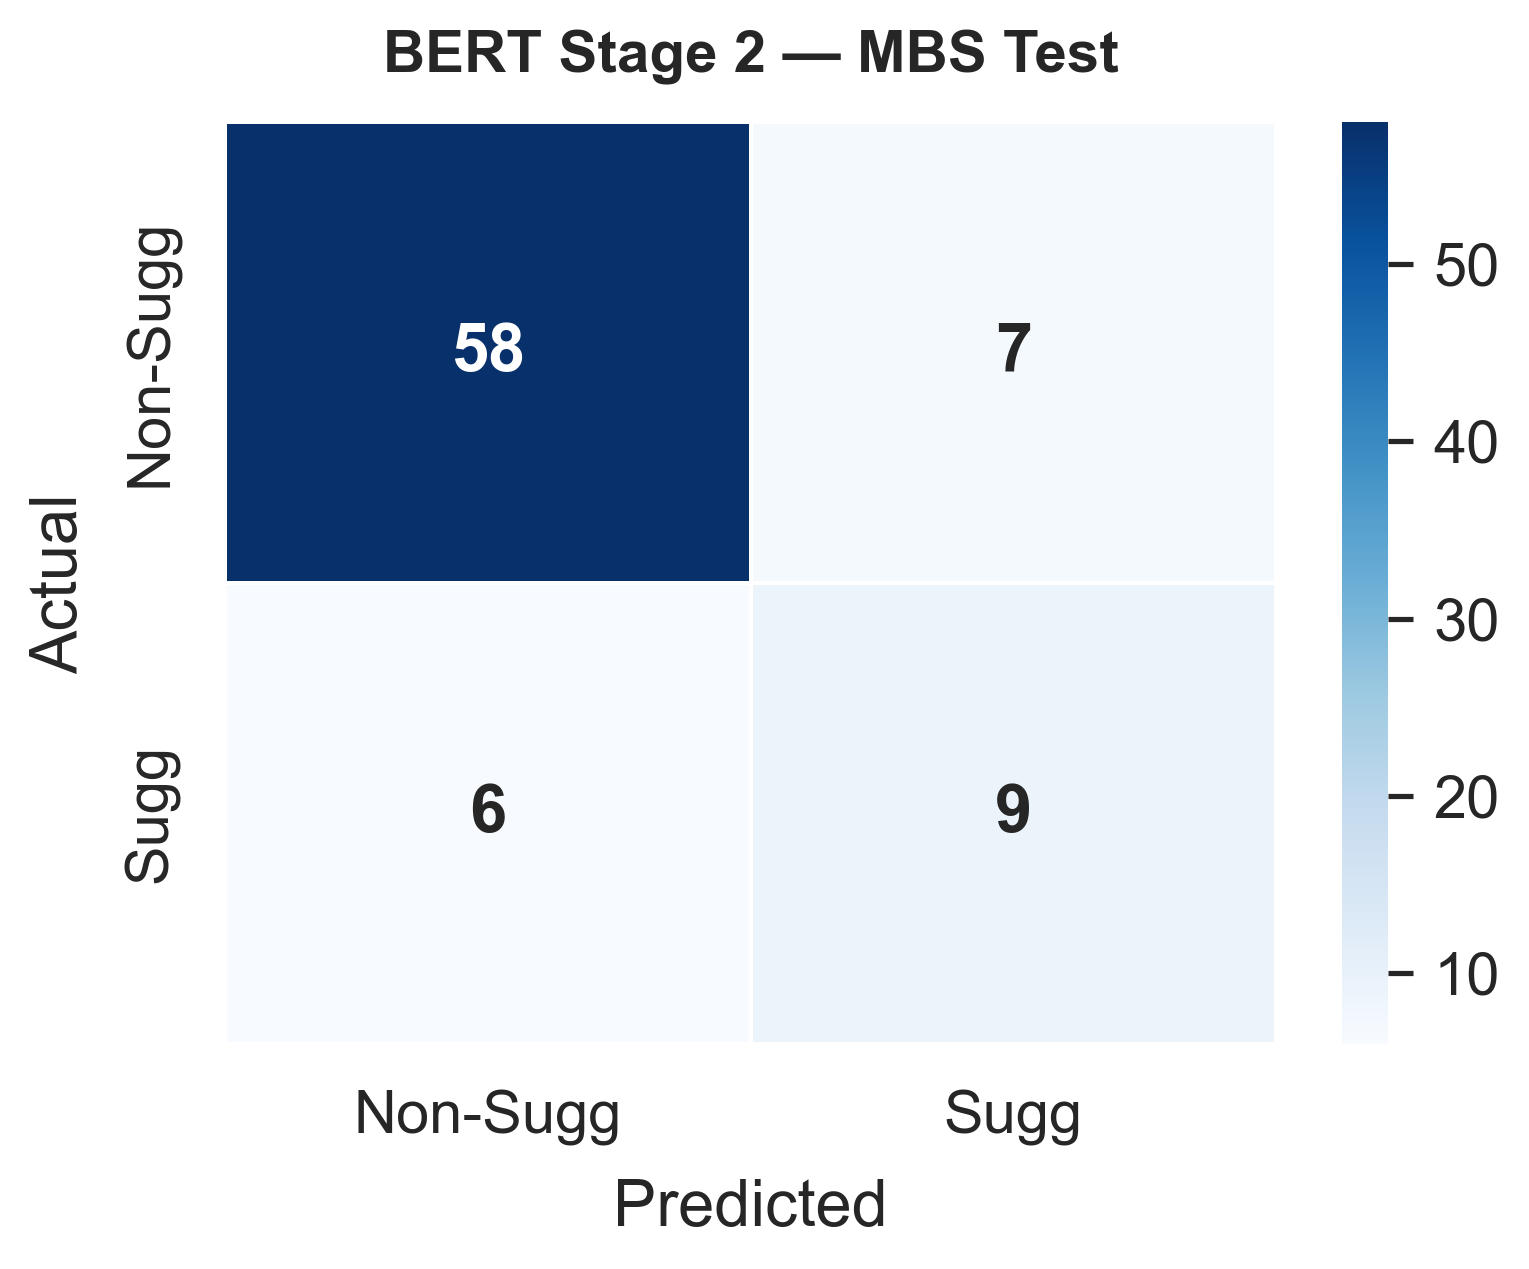
\includegraphics[width=0.75\columnwidth]{cm_bert_s2_mbs.png}
\caption{Confusion matrix for BERT stage-2 on the MBS test
  split (80 sentences).}
\label{fig:cm-s2}
\end{figure}

\subsection{Domain Transfer Analysis}

Cross-domain performance reveals a striking pattern: the two
learned models suffer large drops when moving from SemEval to MBS
(TF-IDF~+~LR: $-$0.406; BERT stage-1: $-$0.430), while the regex
baseline actually improves slightly ($+$0.085). This suggests that
the learned models overfit to SemEval-specific vocabulary and
sentence structures (e.g.\ software feature requests), whereas
simple modal and conditional patterns transfer across domains.
The differing suggestion base rates between the SemEval test set
(10.4\%) and MBS test split (18.8\%) may also partly explain the
regex improvement, as a higher base rate favours
pattern-matching approaches.

However, the regex baseline's cross-domain robustness comes at
the cost of low absolute performance (suggestion-class F1 of
0.471 on MBS). The regex approach generates 11 false positives on
the 80-sentence MBS test split, primarily from positive modal
phrases (e.g.\ ``We would recommend this hotel to anyone'')
that match suggestion patterns but express praise.

BERT stage-2 demonstrates that even a small amount of in-domain
labelled data (320 sentences) can substantially recover
cross-domain performance. Compared to BERT stage-1 on MBS,
stage-2 reduces false negatives from 12 to 6 and improves recall
from 0.200 to 0.600, at the cost of a modest increase in false
positives (3 $\rightarrow$ 7). On the SemEval test set, stage-2
suggestion-class F1 drops from 0.716 to 0.656, with precision
falling (0.624 $\rightarrow$ 0.513) while recall rises (0.839
$\rightarrow$ 0.908)---moderate forgetting from hotel
fine-tuning. Figure~\ref{fig:model-comparison} summarises
suggestion-class F1 across models and datasets.

\begin{figure}[t]
\centering
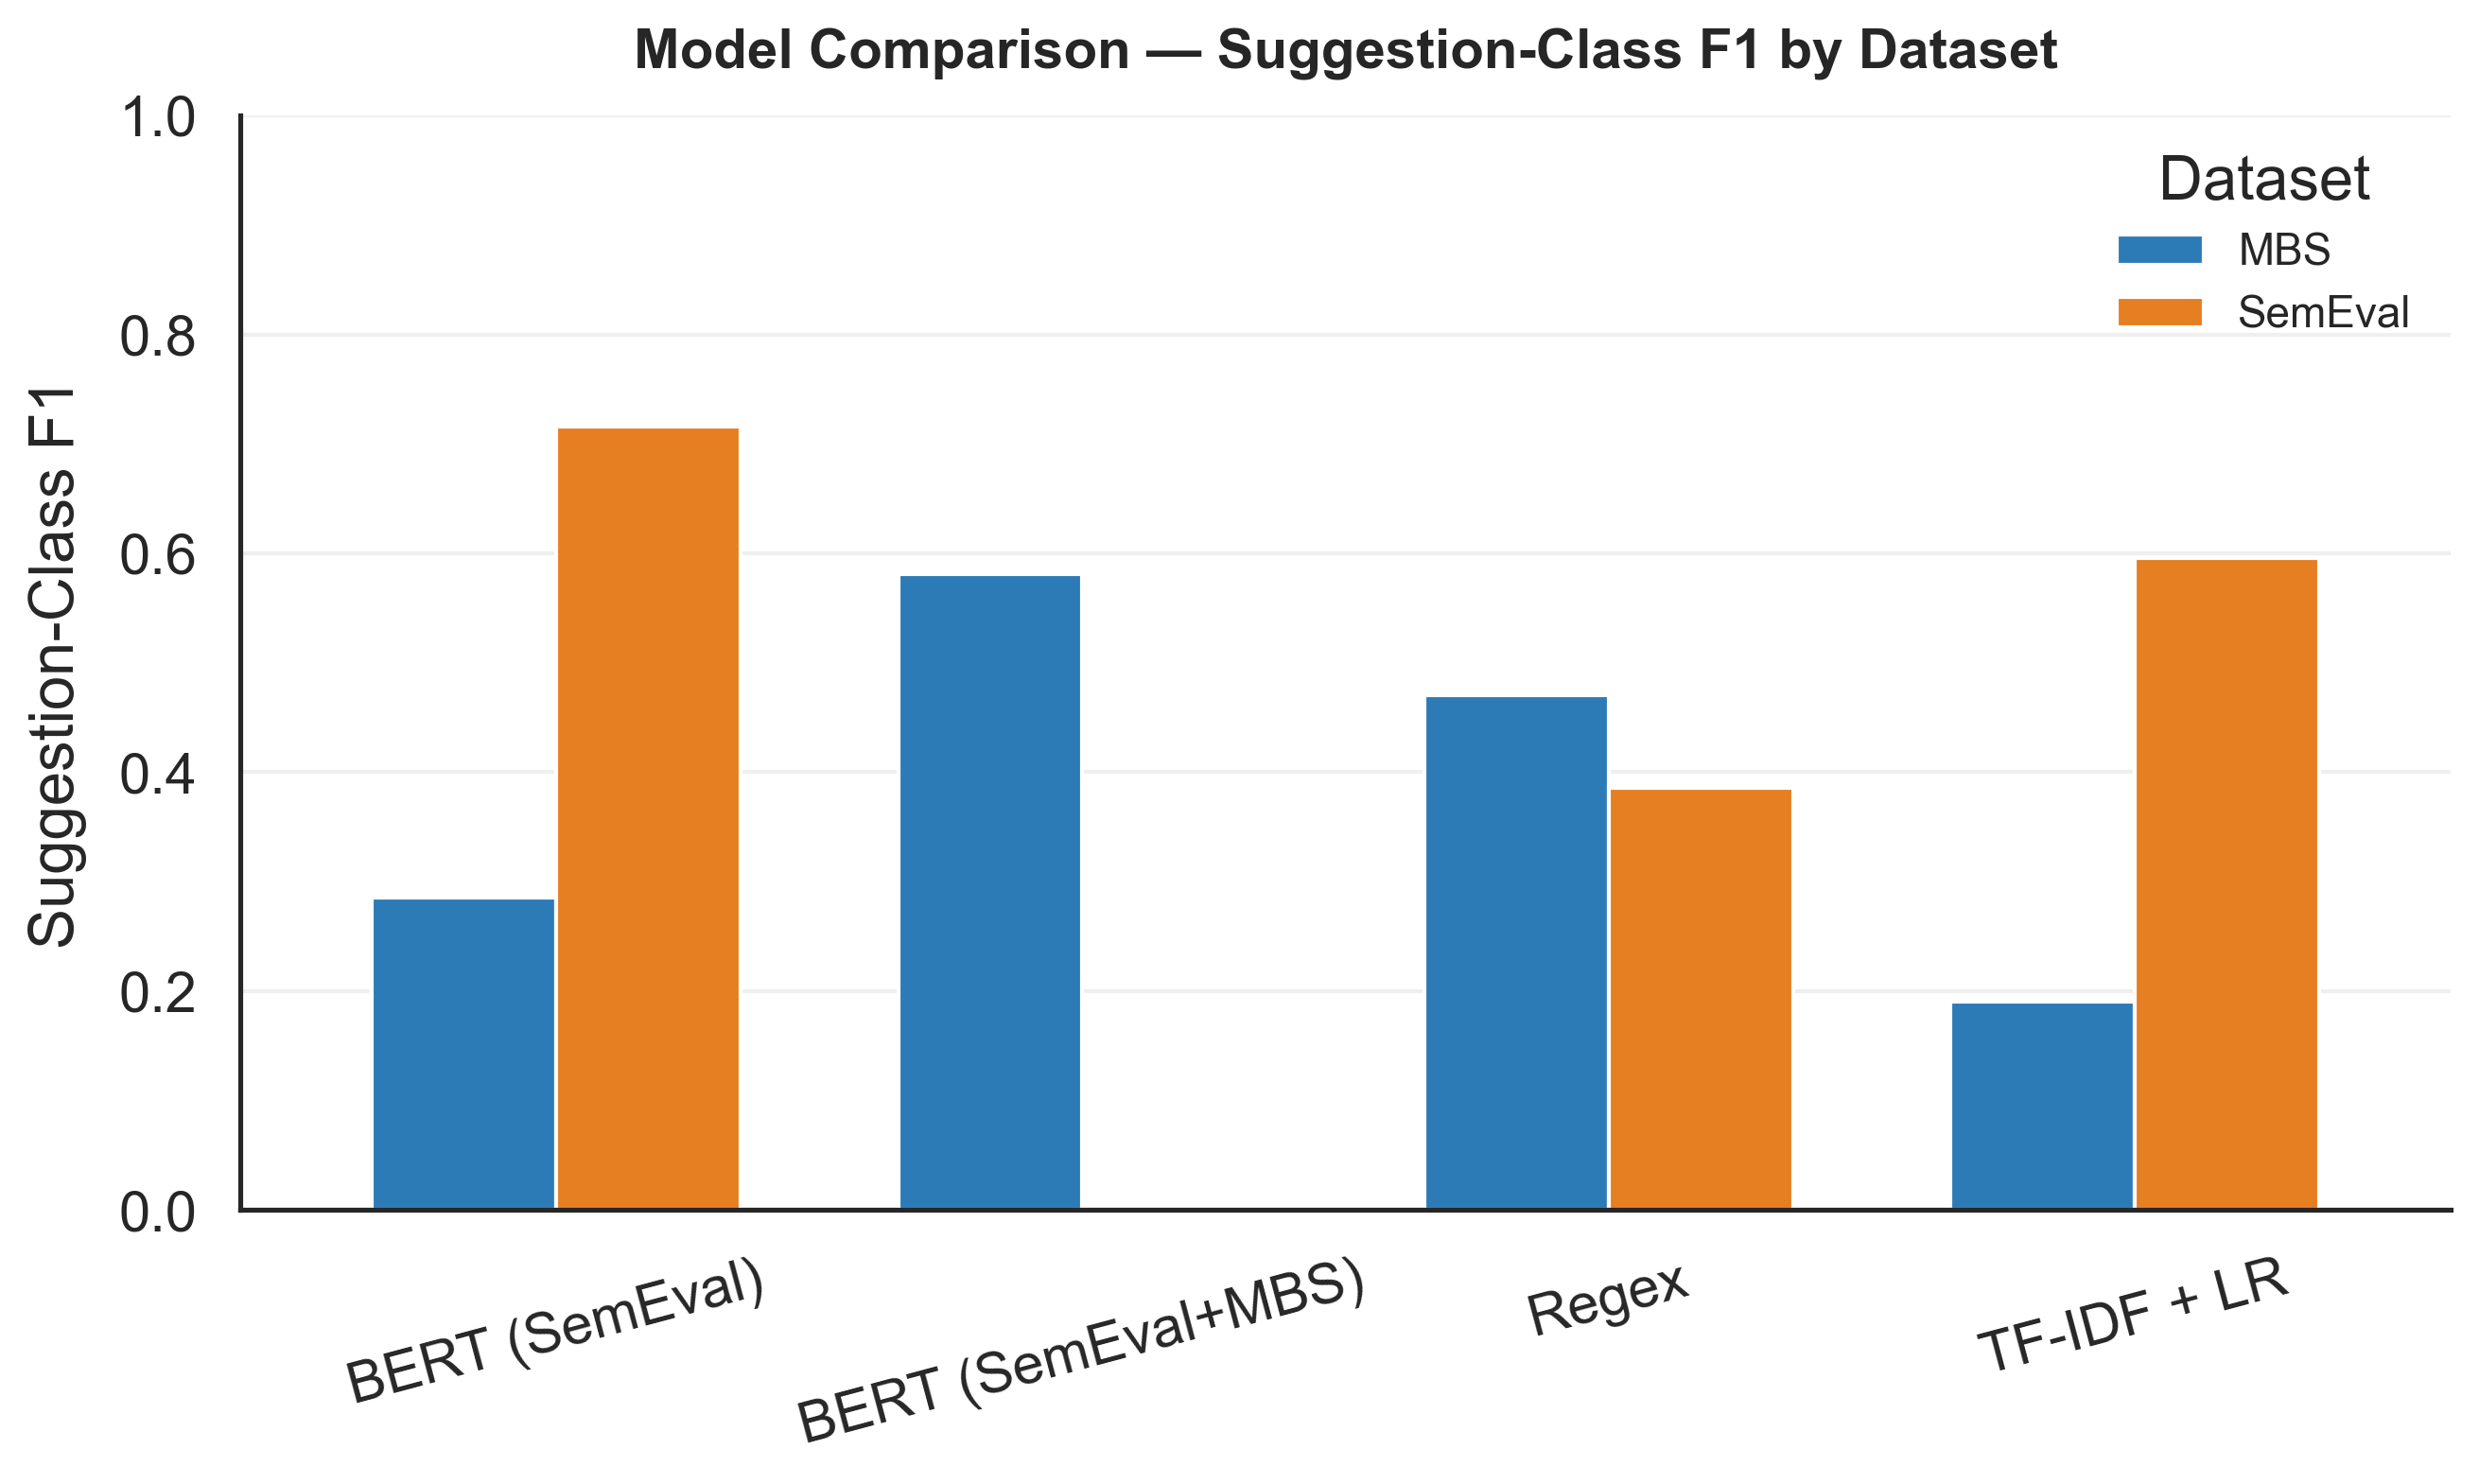
\includegraphics[width=\columnwidth]{model_comparison.png}
\caption{Suggestion-class F1 by model and dataset.}
\label{fig:model-comparison}
\end{figure}

\subsection{Suggestion Themes (BERTopic)}

BERTopic analysis of 4,179 predicted suggestions from BERT
stage-2 identified 56 topics, with topic~0 containing 2,278
sentences and the remaining 55 topics ranging from 5 to 56
sentences each.
Topic~0 functions as a catch-all for sentences lacking
distinctive sub-themes; the finer-grained topics (1--55) capture
specific operational areas such as minibar pricing, elevator
access, and pool amenities.

\begin{table}[t]
\centering\small
\caption{Aspect distribution of predicted suggestions.}
\label{tab:aspects}
\begin{tabular}{lrr}
\toprule
\textbf{Aspect} & \textbf{Count} & \textbf{\%} \\
\midrule
Other            & 1,299 & 31.1 \\
Room             &   990 & 23.7 \\
Facilities       &   638 & 15.3 \\
Food \& beverage &   490 & 11.7 \\
Value            &   309 &  7.4 \\
Service          &   234 &  5.6 \\
Location         &   219 &  5.2 \\
\bottomrule
\end{tabular}
\end{table}

Room-related suggestions dominate (23.7\%), followed by
facilities (15.3\%) and food and beverage (11.7\%). The ``other''
category (31.1\%) captures suggestions that do not match
predefined aspect keywords. Room amenities and physical
facilities together account for 39\% of all detected
suggestions, providing a clear priority for hotel management.

\section{Error Analysis and Discussion}

\subsection{Error Analysis}

We categorise errors from the best-performing model (BERT
stage-2) on the MBS test split using keyword-based heuristics to
assign each sentence to a suggestion type. Of 80 test sentences,
BERT stage-2 produces 7 false positives and 6 false negatives (13
errors total).

\paragraph{False positives.} Five of seven false positives fall
  in the imperative category---sentences containing words like
  ``try'', ``recommend'', or ``please''. These are borderline
  cases: our annotation guidelines (following the SemEval
  definition) classify guest-to-guest advice as suggestions, but
  sentences such as ``We would recommend this hotel to everyone''
  are not improvement-oriented from the hotel's perspective. One
  false positive involves a positive modal phrase, and one has no
  keyword signal. These errors highlight the tension between the
  SemEval suggestion definition (any directive) and the practical
  goal of extracting hotel-relevant insights.

\paragraph{False negatives.} Five of six false negatives belong to
  the ``other'' category---suggestions that lack standard keyword
  signals and instead express improvement needs through
  context-dependent phrasing. The remaining false negative is an
  imperative suggestion. The dominance of the ``other'' category
  among false negatives indicates that hotel review suggestions
  often avoid the explicit modal or imperative language that models
  learn to recognise from the SemEval training set.

\subsection{Domain Gap Discussion}

The cross-domain performance drops observed in
Table~\ref{tab:results} stem from systematic linguistic
differences between software forum posts and hotel reviews.
SemEval suggestions tend to be explicit feature requests (``The
system should allow batch uploads''), using modal verbs and
technical vocabulary. Hotel review suggestions are more often
implicit, embedded within narrative praise or complaints (``I wish
the breakfast had more variety''), and use hospitality-specific
language absent from the SemEval training set.

The learned models (TF-IDF~+~LR and BERT stage-1) overfit to
SemEval-specific patterns, resulting in high false-negative rates
on MBS (13 and 12 out of 15 suggestions missed, respectively).
The regex baseline, by contrast, relies on domain-general modal
and conditional patterns that transfer across domains, explaining
its slight improvement on MBS ($+$0.085 suggestion-class F1).

BERT stage-2 partially closes the domain gap. With only 320
in-domain training sentences, it recovers suggestion-class recall
from 0.200 (stage-1) to 0.600 (stage-2), while maintaining
precision at 0.563. This trade-off is visible in the error
comparison: stage-2 reduces false negatives from 12 to 6 but
increases false positives from 3 to 7. In practice, higher recall may be preferable, as
missing genuine suggestions is costlier than reviewing a few
false positives. Figure~\ref{fig:error-comparison} summarises the
FP/FN trade-off across all four models.

\begin{figure}[t]
\centering
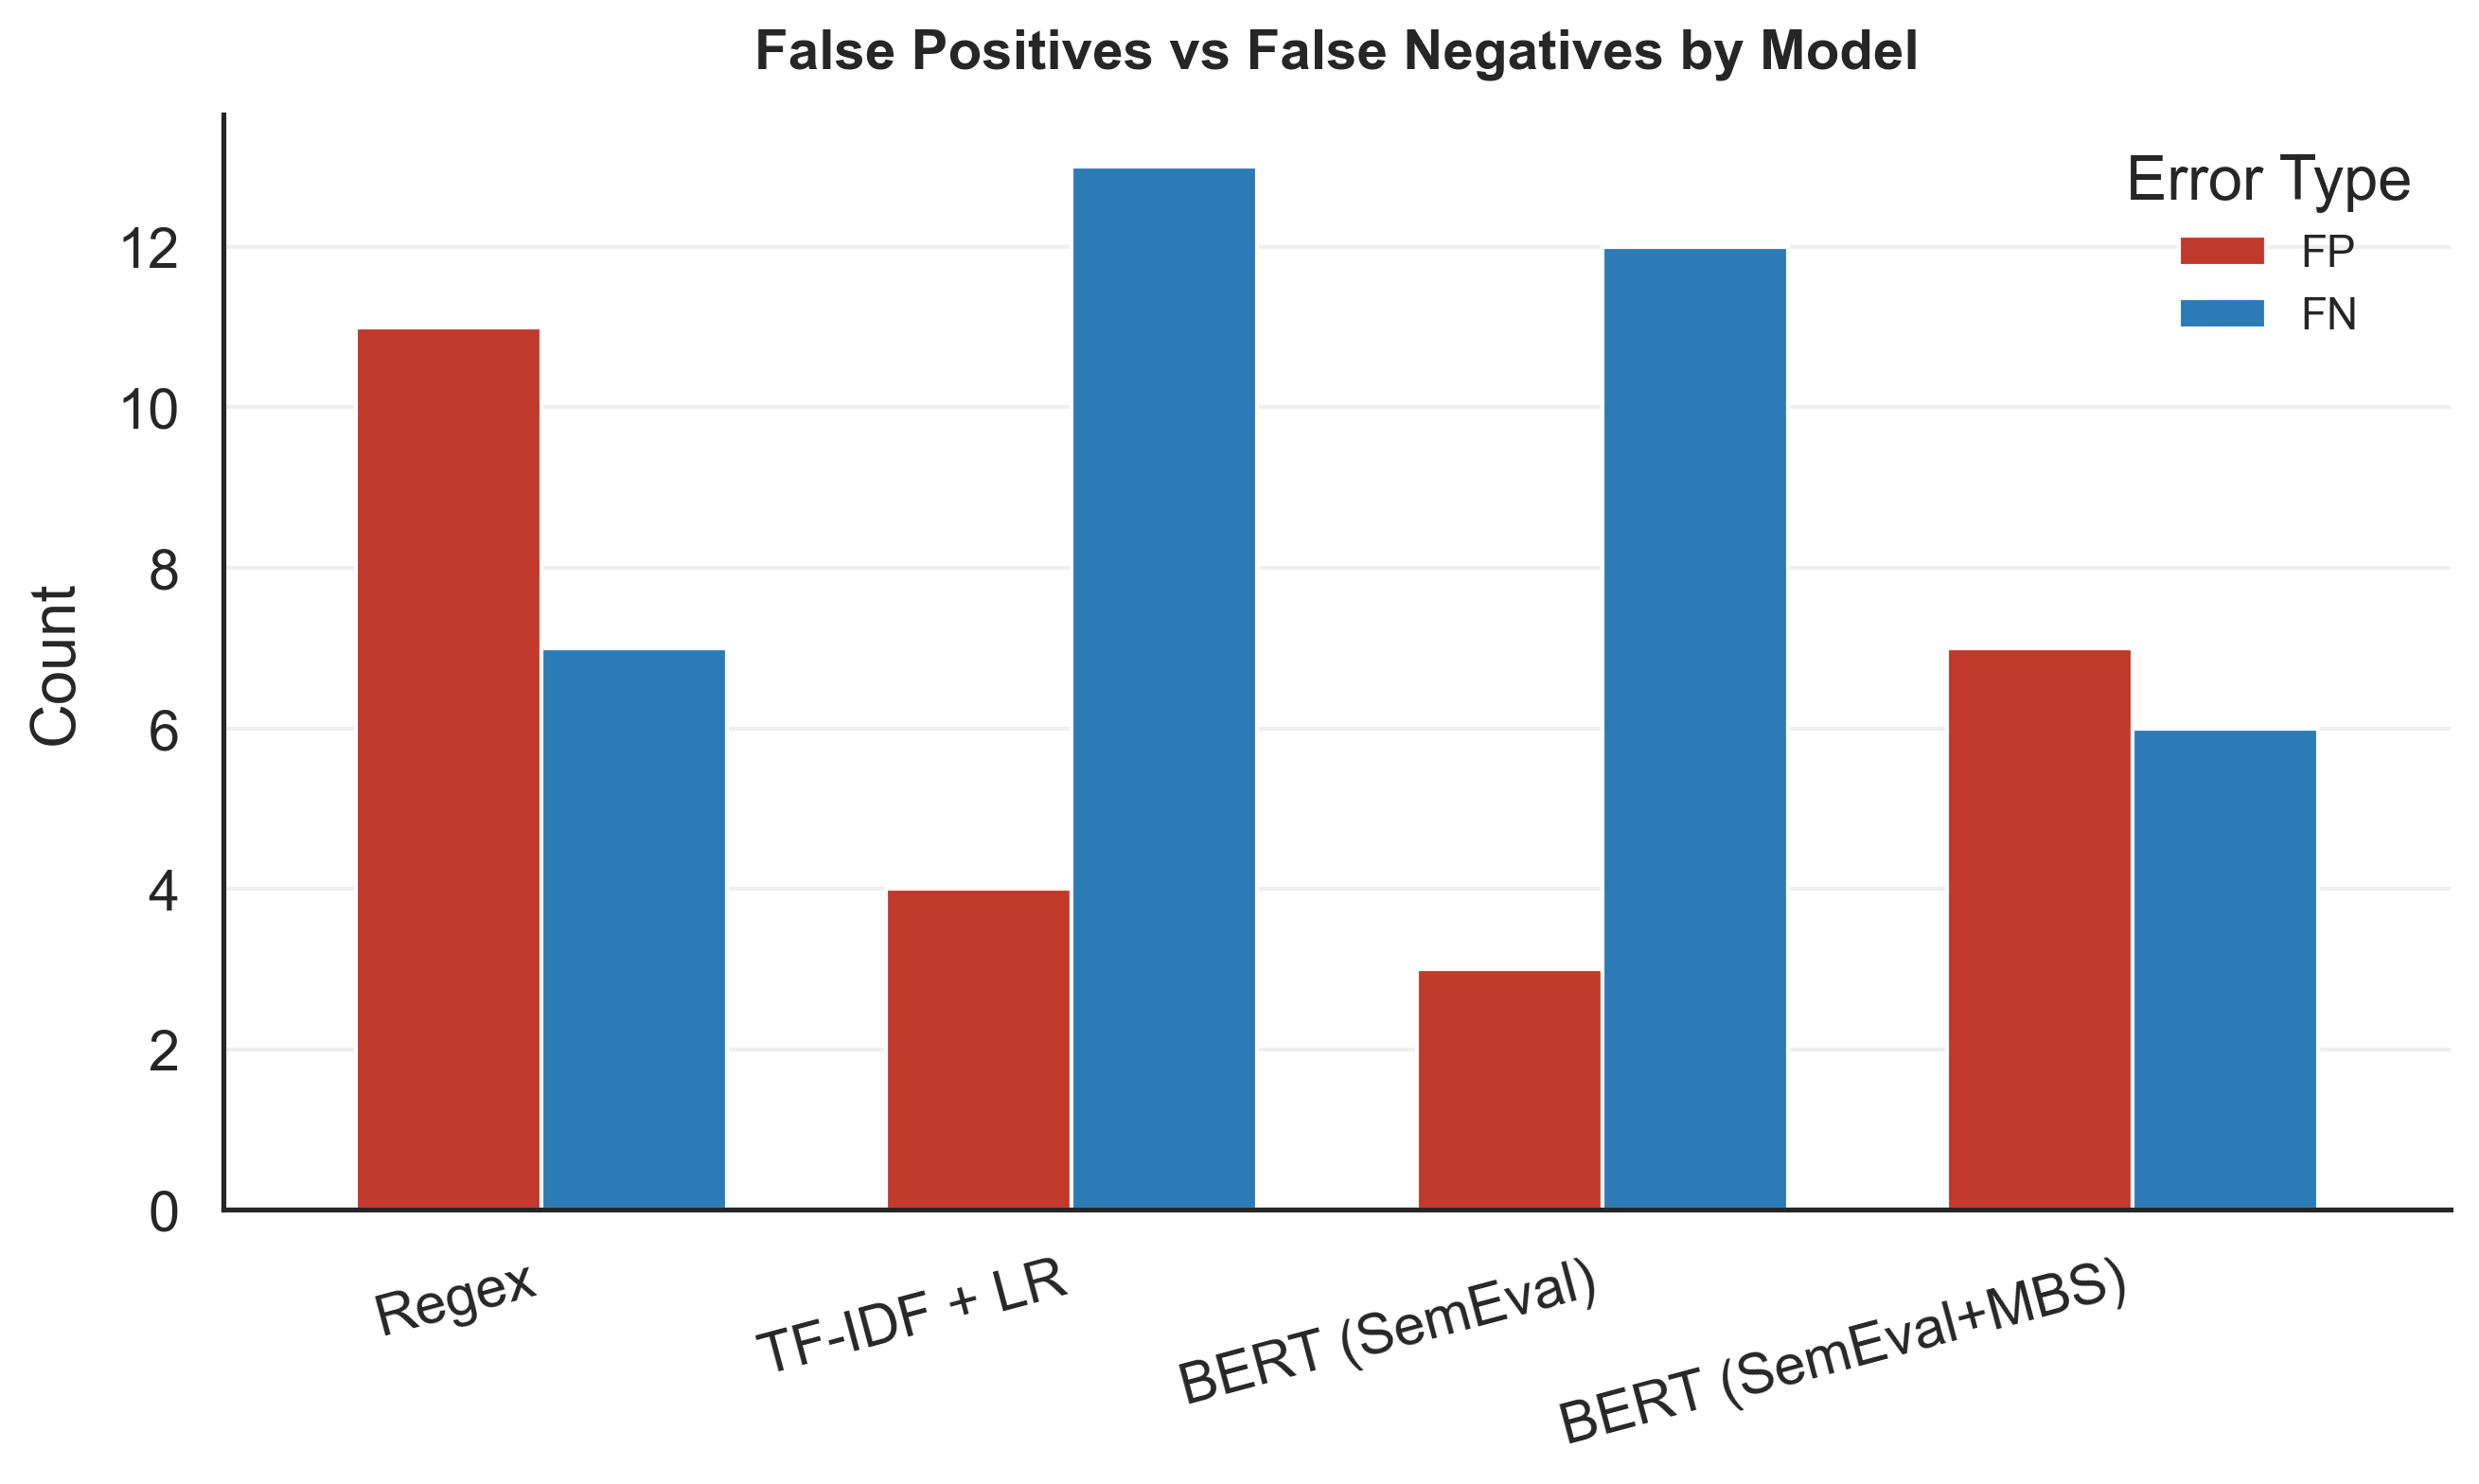
\includegraphics[width=\columnwidth]{error_comparison_models.png}
\caption{False positives versus false negatives by model on the
  MBS test split. Stage-2 fine-tuning shifts the error profile
  from FN-dominant to more balanced.}
\label{fig:error-comparison}
\end{figure}

\subsection{Limitations}

\begin{itemize}
  \item \textbf{Annotation scale.} The MBS annotated set contains
  400 sentences, with a test split of only 80 sentences (15
  suggestions). Metrics on this test split have wide confidence
  intervals; a single additional correct prediction would shift
  suggestion-class F1 by approximately 0.05. We did not compute
  bootstrap confidence intervals, so reported differences should
  be treated as indicative rather than statistically confirmed.
  \item \textbf{Single hotel.} All MBS data comes from one
  property. Generalisability to other hotels or hospitality
  segments is unknown.
  \item \textbf{Annotation subjectivity.} Fleiss' $\kappa$ of
  0.379 indicates fair but not strong agreement. The boundary
  between complaints and suggestions is inherently fuzzy, as
  reflected in the 11 calibration ties. Furthermore, 300 of 400
  annotated sentences were labelled by a single annotator each,
  with no inter-annotator validation on these split batches.
  \item \textbf{No human upper bound.} We did not compute
  human--model agreement on the test split.
  \item \textbf{Sentence isolation.} Each sentence is classified
  independently, without review-level context. Suggestions that
  span multiple sentences may be missed.
  \item \textbf{No manual validation.} We did not manually
  validate predictions on the full 70,085-sentence MBS dataset.
  The thematic analysis in Section~5.3 relies on BERT stage-2
  predictions, which achieve suggestion-class F1 of 0.581 on the
  MBS test split but may still contain systematic errors at
  scale.
\end{itemize}

\subsection{Future Directions}

\begin{itemize}
  \item Annotate 1,000+ sentences to reduce test-split variance.
  \item Include multiple hotels for cross-property generalisation.
  \item Investigate few-shot or prompt-based approaches using large
  language models as alternatives to fine-tuning.
  \item Use sentence-pair context to detect implicit suggestions
  that depend on surrounding text.
\end{itemize}

\section{Conclusion}

To what extent can NLP models detect actionable improvement
suggestions within high-star hotel reviews? Our experiments show
that suggestion mining is feasible in the hotel review domain, but
cross-domain transfer from software forums degrades substantially
without domain adaptation. BERT stage-2, fine-tuned on just 320
hotel-domain sentences, achieves suggestion-class F1 of 0.581 on
the MBS test split---approximately double the cross-domain-only
result (0.286) and the best performance among all models tested.

Our contributions are:
\begin{enumerate}
  \item Domain-adapted annotation guidelines for hotel review
  suggestions, validated with Fleiss' $\kappa$ of 0.379 on a
  100-sentence calibration sample across four annotators.
  \item A three-tier model comparison demonstrating that
  contextual representations (BERT) outperform bag-of-words
  features (TF-IDF~+~LR, suggestion-class F1 0.596) and surface
  patterns (regex, 0.386) on in-domain data, but that this
  advantage does not automatically transfer cross-domain.
  \item Two-stage fine-tuning that improves MBS suggestion-class
  F1 by 0.295 points (from 0.286 to 0.581), recovering recall
  from 0.200 to 0.600 with only 320 in-domain training sentences.
  \item Thematic analysis of 4,179 predicted suggestions (from
  BERT stage-2, suggestion-class F1 = 0.581) indicating that
  room-related suggestions account for the largest share
  (23.7\%), followed by facilities (15.3\%) and food and
  beverage (11.7\%). At precision 0.563, roughly 44\% of inputs
  to BERTopic may be false positives, so these distributions are
  approximate.
\end{enumerate}

Future work should scale annotation to more hotels and review
platforms, investigate prompt-based suggestion detection using
large language models, and explore multi-label classification of
suggestion types (explicit, implicit, comparative).


\bibliography{references}

\appendix
\section{Annotation Guidelines Summary}
\label{app:guidelines}

Each sentence is labelled as suggestion~(1) or
non-suggestion~(0). The core decision rule is: ``Does this
sentence propose a concrete action the hotel could take to
improve?'' Guidelines cover six edge-case categories:

\begin{enumerate}
  \item \textbf{Wishes and desires} (label~1): ``I wish the pool
  was open later'' implies extending pool hours.
  \item \textbf{Implicit comparisons} (label~1): ``Other hotels
  offer free shuttle'' implies adding a shuttle service.
  \item \textbf{Conditional praise} (label~1): ``Great hotel, but
  they need to fix the elevators'' contains an actionable clause.
  \item \textbf{Complaints without direction} (label~0): ``The
  check-in took over an hour'' describes a problem without
  proposing a fix.
  \item \textbf{Positive modals} (label~0): ``I would definitely
  stay again'' uses ``would'' for praise, not suggestion.
  \item \textbf{Guest advice} (label~1): ``Try the laksa at the
  food court'' is a recommendation with a directive element.
\end{enumerate}

Guidelines were revised (v1.0 $\rightarrow$ v1.1) after the
calibration round to clarify the complaint-versus-suggestion
boundary and the distinction between informational statements
and guest-directed advice.

\section{Code Availability}
\label{app:code}

All code, data processing scripts, and trained model checkpoints
are available at
\url{https://github.com/LanscorTK/NLP_Team6}. The full
pipeline can be reproduced with
\texttt{python run\_pipeline.py}.

\section{AI Tool Acknowledgement}
\label{app:ai}

We used Claude (Anthropic) as an assistive tool for coding
support and project planning throughout this project. Specific
uses included: debugging Python pipeline code, drafting
boilerplate LaTeX structure, and literature search assistance
via arXiv and Semantic Scholar API integrations. All substantive
research decisions---task formulation, annotation guideline
design, model selection, hyperparameter choices, and
interpretation of results---were made by the team. Claude was
not used to generate report prose; all analytical writing was
authored by team members. This disclosure follows UCL guidance
on acknowledging the use of generative AI tools in assessed
work.


\end{document}
